\justifying
\NSFCBodyText

% \subsubsection{研究背景}

% \subsubsubsection{案例概述}
% 佐佐木希（Nozomi Sasaki，1988年生）作为日本演艺产业代表性人物，其职业生涯从2002年持续至今，跨越模特、演员、歌手等多领域。2002年获全日本国民美少女比赛模特组冠军出道，初期活跃于《Pinky》《Non-no》等时尚杂志。2008年起向影视转型，出演《热血街区》等作品。2010年代拓展至综艺、音乐领域。2020年面对丈夫出轨风波，采取“沉默—原谅—重启”策略修复公众形象。2024年开设个人YouTube频道，开启新媒体转型。

% \subsubsubsection{研究价值}
% 佐佐木希的职业发展路径为理解东亚娱乐产业变迁、女性艺人转型策略及跨媒介形象管理提供了极具价值的案例。其职业生涯跨越日本娱乐产业从传统媒体向新媒体转型的关键期（2005-2025）。作为女性艺人，她面临的性别化挑战具有典型性。2020年个人危机处理案例为研究品牌韧性机制提供了珍贵实证。

% \subsubsubsection{研究问题}
% 本研究旨在通过系统分析佐佐木希近20年职业轨迹，探讨：（1）艺人职业转型期关键节点识别；（2）跨媒介形象构建的动态机制；（3）个人品牌在不同生命周期阶段的价值维持策略。

% \subsubsection{国内外研究现状}

% \subsubsubsection{职业转型理论}
% 目前研究主要集中三个方向：Smith（2020）提出“职业锚理论”\cite{Smith2020}；Super（1957）划分职业发展五阶段\cite{Super1957}，但缺乏东亚语境研究。

% \subsubsubsection{形象管理研究}
% Johnson（2019）提出“建构—维护—修复”三阶段\cite{Johnson2019}；Goffman（1959）的“自我呈现”理论\cite{Goffman1959}，但新媒体环境研究不足。

% \subsubsubsection{产业生态分析}
% Tanaka（2021）比较日韩艺人培养体系\cite{Tanaka2021}；Jin（2016）分析韩国产业全球化\cite{Jin2016}，但个体定位策略研究匮乏。

% \subsubsection{现有研究的局限性}

% \subsubsubsection{理论层面}
% 现有研究存在以下不足：（1）缺乏完整职业生命周期的纵向案例研究；（2）对个人品牌韧性机制探讨不足；（3）忽视女性艺人的特殊挑战。

% \subsubsubsection{方法层面}
% （4）未能充分整合跨学科视角；（5）新媒体环境下艺人-粉丝关系重构研究不足。

% \subsubsection{研究切入点}

% \subsubsubsection{案例独特性}
% 佐佐木希的职业轨迹具有独特研究价值：（1）转型涵盖“模特→演员→歌手→综艺艺人→YouTuber”完整链条；（2）经历2020年个人危机的形象修复过程；（3）职业发展与产业变迁高度同步。

% \subsubsubsection{研究代表性}
% （4）从地方到全国性的典型路径；（5）女性艺人的性别化挑战具有代表性。


% 面向人机共融的高表现力具身智能感知与生成机制研究

% (6-8页，占比20\%-27\%,。
% \textbf{需要减少的内容：}铺垫研究合理性，服务核心内容。砍掉无价值铺垫，背景科普等评审专家认知深刻内容，2-3句话带过即可，无需整页科普。无需梳理领域完整发展脉络，仅保留与本研究直接相关、支撑科学问题提出的核心文献，剔除无关综述内容。30-50篇核心文献足够，关键是每篇均与研究强相关，无需七八十篇文献凑数，避免文献列表占用2-3页。研究意义无需在开头、中间、结尾反复强调，一次精准表述即可。弱相关"国家需求"铺陈:无需5页空泛论述领域重要性，直接切入核心问题，规避铺陈式误区。
% \textbf{需要弄清楚的内容：} 
% 立项依据的核心是"漏斗式聚焦":从宽泛背景逐步收窄至具体、清晰、有价值的科学问题，这一过程需写透，占比超一半篇幅，
% 重点厚在三方面:
% 正面示例(穿透式开篇):300字直击核心--领域当前"卡点"(Gap)是什么?现有方法的局限的?本研究核心思路(Keyldea)如何精准突破?
% 负面示例(铺陈式开篇):花5页讲领域重要性，3页罗列他人成果，迟迟不切入核心科学问题
% )

\subsubsection{研究意义与国家战略需求}

服务机器人已具备基础的场景导航与物体操作能力，但在与人类情感韵律相协调的非语言行为（Non-verbal Behavior）表达上仍普遍欠缺。心理学与人机交互领域的研究表明，面对面交流中超过60\%的信息传递依赖面部表情、手势节律与躯干姿态等副语言信号~\cite{mehrabian1971silent}。这一能力缺口使人机交互过程显得机械、割裂，构成了具身智能在适老化陪护、医疗康复等非结构化社会民生场景中落地的关键瓶颈，限制了应用范围。

突破上述交互认知瓶颈与国家战略高度契合。党的二十届三中全会通过的《中共中央关于进一步全面深化改革 推进中国式现代化的决定》明确提出加强未来产业前瞻布局；工信部《人形机器人创新发展指导意见》~\cite{MIIT2023}与工信部等七部门于2024年联合发布的《关于推动未来产业创新发展的实施意见》中，将``突破机器人大脑认知与小脑控制协同瓶颈，构建高可靠、高交互的人机共融系统''列为核心攻关任务~\cite{MIIT2024Future}。2024年《政府工作报告》首次提出``人工智能+''行动~\cite{GovReport2024}，指向生成式大模型从数字内容生成向物理实体赋能的跨越；自“十五五”规划~\cite{Gov2025155}至《人形机器人与具身智能标准体系（2026版）》~\cite{humaoid2026}，政策对具身智能与机器人的支持持续加码。上述部署直指本项目要解决的核心难题：如何使实体机器人超越冰冷指令执行，理解复杂社交语境，并以高表现力、拟人化的肢体语言作出自然反馈。

民生侧，我国人口老龄化加剧，国务院办公厅《关于发展银发经济增进老年人福祉的意见》~\cite{SilverEcon2024}指出，居家养老与机构陪护场景中老年群体对智能装备的需求已由单一物理辅助延伸至深层情感慰藉。现有服务机器人在移动导航与机械抓取上已初步成熟，多模态情感表达却仍存在明显空白；``有执行力、无共情力''的现状不仅难以消弭人机交互中的``恐怖谷效应''，反而易加重使用者的认知负荷与排斥心理~\cite{qiao2022brain}，阻碍老年群体与机器人建立长期情感信任。

理论层面，北京航空航天大学陆峰教授与赵沁平院士提出的``共身智能（Cobodied/Symbodied AI）''理念~\cite{lu2025cobodied}为突破上述交互瓶颈提供了系统性框架：下一代智能体应从以物理环境适应为核心的``具身''，演进为以人机认知对齐为目标的``共身''，通过跨智能体的语义对齐与物理协同实现真正的人机共融。本项目立足该视角，针对高移动稳定性的履带式上半身人形机器人构型，探究面向共身智能的高表现力社交动作感知与生成机制，从科学机理上阐明：\textbf{跨模态情感语义如何有效跨越虚实鸿沟，驱动受限于动力学边界的刚性机器人实体，呈现出柔性、共情且符合人类社会交互规范的高表现力行为。}

\subsubsection{国内外研究现状与发展动态分析}

围绕具身智能交互与高保真动作生成，国内外学者近年来开展了大量前沿探索。然而，面向真实物理实体的高表现力社交动作生成，仍横跨机器人学与计算机图形学，面临诸多学科交叉维度的理论空白。

\noindent{\textbf{1. 具身控制与VLA大模型：物理操作精细，但社交语义贫瘠。}}
在具身机器人的端到端控制领域，``视觉-语言-动作（VLA）''范式已展现出强大的泛化潜力。从早期的RT-2~\cite{brohan2023rt2}，到近期开源的Octo~\cite{octo2024}与OpenVLA~\cite{kim2024openvla}，研究者通过联合训练视觉语言模型与机器人轨迹，实现了对未见物体与指令的零样本泛化。更进一步，结合扩散策略（Diffusion Policy）~\cite{chi2023diffusion}与流匹配（Flow Matching，如$\pi_{0.5}$等工作~\cite{Intelligence2025}）的最新物理智能架构，显著提升了多步任务序列生成的连续性与多模态对齐精度。

上述VLA工作的数据与目标却高度同质：绝大多数依赖遥操作（Teleoperation）采集的大规模数据集（如Open X-Embodiment~\cite{padalkar2024open}），操作员注意力集中于末端执行器（End-effector）位姿精度，数据中因而极少包含面部表情、头部注视与自然肢体伴随动作。现有动作标注以``物理任务完成率''为单一目标，情感意图刻画不足，头-面-手-躯干的多部位协同机制尚未建立；面对``对低落情绪做出安抚反馈''等复合社交指令，现有框架对副语言信息的表征能力不足，暴露出具身控制基座在情感感知与非语言行为维度的系统性贫瘠。

\noindent{\textbf{2. 语音驱动的数字人生成：情感表现力丰富，但缺乏物理真实性。}}
与之形成鲜明对比的是，在计算机图形学与虚拟数字人领域，由语音与文本驱动的高表现力动作生成技术已日趋成熟。借助SMPL-X~\cite{pavlakos2019expressive}等参数化模型的统一表达，学术界已能从海量单目互联网视频中提取高质量的交互数据。从早期的规则与自回归生成~\cite{ginosar2019learning}，到近年来基于扩散模型的生成算法（如DiffSHEG~\cite{Chen2024DiffSHEG}、MODA~\cite{Liu2023MODA}与EMAGE~\cite{liu2024emage}），实现了从语音音频到面部表情、手势甚至精细手指动作的高保真协同生成，在数字空间中达到了以假乱真的表现力。

尽管在视觉感知层面表现优异，但此类算法生成于无物理约束的纯运动学空间。其生成的动作流形往往存在关节角速度超限、不可实现的质心加速度以及严重的自碰撞问题。当这些基于纯几何生成的动作序列通过传统逆运动学（IK）映射至真实机器人时，极易因忽略电机峰值力矩与底盘动力学平衡，导致硬件过载、动作严重失真或触发急停保护~\cite{wang2023intelligent}。

\noindent{\textbf{3. 虚实迁移与重定向：追求动力学稳定，却造成表现力折损。}}
为跨越``虚实鸿沟''，基于强化学习（RL）的物理级虚实迁移（Sim-to-Real）成为自然选择。依托NVIDIA Isaac Lab~\cite{nvidia2023isaac}等高保真仿真环境进行物理智能训练，OmniH2O~\cite{he2024omnih2o}与PHC~\cite{luo2023phc}等实现了人体动捕数据驱动人形机器人全身模仿；Mobile ALOHA~\cite{fu2024mobilealoha}与HumanPlus~\cite{li2024humanplus}则验证了从人类运动视频学习全身操作策略的可行性。

然而，现有RL追踪框架多侧重于双足行走（Locomotion），基础操作平衡，或者末端抓取，其奖励函数通常对高动态的关节加速度与质心偏移施加严厉的惩罚项。这种保守的控制策略在面向``高动态情感社交动作''（如激动地挥手、前倾大笑）时，会强制将大幅度的柔性动作``抑制''为小幅度的僵硬动作，以换取底盘的绝对稳定。这种缺乏底盘协同抗扰动设计的重定向机制，导致源数据中丰富的情感语义与节律特征在跨平台映射中被系统性折损。

综上所述，现有研究在面向\textbf{``物理可行的高表现力社交动作生成''}这一交叉领域存在明显断层：具身智能VLA模型缺乏社交共情数据与属性建模；图形学生成方法缺乏物理动力学闭环约束；而现有的物理重定向技术又以牺牲情感表现力为代价换取稳定性。此外，在生成机制底层，离散的意图理解模型与连续的物理动作流形之间，尚未建立起严格的时空对齐理论。本项目正是针对这一交叉空白，提出面向共身智能的社会化多模态语言动作生成架构（Social Multi-modal Language-Model based Action generation，Social-MLA），系统建立从感知解耦、物理映射到协同生成的完整科学研究框架。

%-------------------------------------------------------------------------
% 插入图1：项目总体研究思路示意图
%-------------------------------------------------------------------------
\begin{figure}[htbp]
    \centering
    % 请确保图片路径与文件名正确
    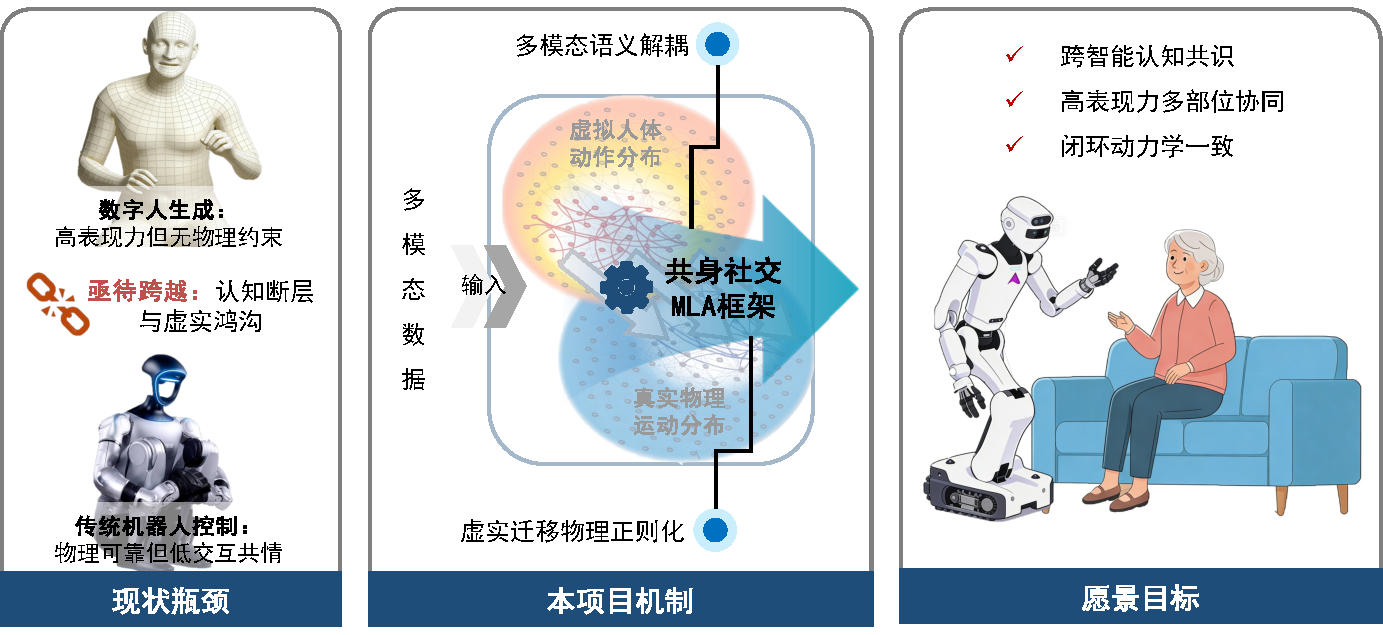
\includegraphics[width=\linewidth]{figures/overall-motivation.pdf}
    \caption{\textbf{项目总体研究思路与科学逻辑示意图。} 针对当前具身智能领域“懂物理操作但缺社交共情”的痛点，以及图形学数字人生成面临的“虚实鸿沟”，本项目提出面向人机共融的高表现力共身智能感知与生成机制（共身社交MLA）。通过在特征空间对齐虚拟动作分布与真实物理约束，建立异构实体的认知-动作映射与物理级虚实迁移，赋予履带式人形机器人高表现力的社会化交互能力，实现人机在物理实体与认知语义层面的双重共融。}
    \label{fig:concept}
\end{figure}

\subsubsection{拟解决关键科学问题}

结合上述学科瓶颈与共身智能感知与生成（Social-MLA）技术路线，本项目在多模态感知解析、非线性异构映射与跨模态协同生成三个层面拟解决以下递进的关键科学问题：

\begin{enumerate}
    \item \textbf{复杂交互语境下多维非语言行为特征的时空同步解析与解耦机理}

    自然的人机或人人对话中，面部微表情、视线焦点与肢体手势高度时序耦合，视觉捕获时又常遇严重自遮挡与互遮挡。现有基于参数化人体模型的单向估计缺乏部位间联合先验，难以剥离多部位协同的深层意图规律。核心科学问题在于：在分析-合成（Analysis-by-Synthesis）范式下，如何突破独立特征提取的局限，建立``表情-视线-动作''多维特征在复杂动态条件下的时空同步解析模型，并探明各特征在情感表达中的权重与耦合规律，为下游任务生成提供兼具物理真实性与高判别性的感知先验？

    \item \textbf{受限物理实体约束下的非线性拓扑映射与动力学边界补偿机制}

    将高达145个自由度的柔性人体动作重定向至低自由度刚性履带式人形机器人时，拓扑异构与执行器动力学极限（关节力矩峰值、底盘倾覆力矩等）会使传统一对一运动学映射（Motion Retargeting）严重失效，造成动作情感语义的结构性折损。要解决的核心科学问题在于：如何突破传统静态逆运动学解算的局限，将高保真物理仿真中的碰撞与动力学反馈作为隐式正则项纳入映射优化闭环，并在此基础上建立约束流形上的非线性映射理论，实现``社交语义关键帧保真度''与``机器人动力学可行域''的联合最优？

    \item \textbf{离散语义Token驱动下的连续具身动作流形跨模态演化机理}

    高表现力交互动作需同时满足高层情感逻辑的离散结构与底层关节物理控制的连续平滑；自回归大模型长于离散Token序列，流匹配（Flow Matching）等则长于连续动作分布流形，二者在模态表征上存在深层鸿沟。核心科学问题即：在融合大语言模型与常微分方程（ODE）求解的混合架构下，如何建立离散多模态交互Token序列对ODE连续演化轨迹的有效引导与调制机制，揭示解码过程中跨模态表征的对齐规律，使生成的动作轨迹既符合语义空间的离散指令意图，又严格收敛于安全平滑的动力学边界内？
\end{enumerate}
